\documentclass{standalone}
\begin{document}
	\subsection{Color Quantization}
	

	Color quantization is the process of reducing the number of colors in a digital image. The main objective of quantization process is that 
	significant information should be preserved while reducing the number of colors in an image, in other word quantization process shouldn’t cause 
	significant information loss in the image. 
	Color quantization, accepted as a pre-processing application, is used to reduce the number of colors in images with minimum distortion such that the 
	reproduced image should be very close to the original image visually, as in \figurename\,\ref{fig:ColorQuantization}. 

	\begin{figure}[h!]
		
		\centering
			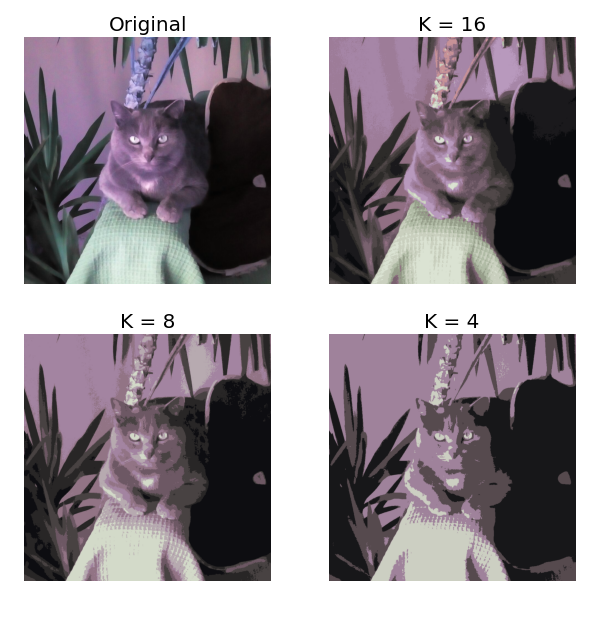
\includegraphics[scale=.6]{ColorQuantization.png}
		\caption{\textit{Color quantized RGB image. We observe the original image, a 16 color image which look similar to the original one, a 8 colors image and 4 colors image}}\label{fig:ColorQuantization}
	\end{figure}

	Color quantization play an important role in many filed of applications such as segmentation, compression, color texture analysis, watermarking, 
	text localization/detection, non photorealistic rendering and content-based retrieval~\cite{ART:Ozturk}.\\
	
	
	Color quantization may be used for image segmentation. Use that for this purpose means to reduce the number of colors to the number of the different objects we seek to segment. This means that is is based on the assumption that to each different object class in the image is assigned an unique characteristic color. This is the case of image segmentation, in which each image color represent a particular characteristic of the tissue displayed(i.e in x-ray represent$\mu$). 
	To perform this technique, different algorithms may be used to group the colors, like clustering algorithm or the principal component analysis.


	
	
	
	

	
	
\end{document}